\documentclass[a4paper,12pt]{article}
\usepackage[fleqn]{amsmath}
\usepackage{amssymb}
\usepackage{graphicx}
\graphicspath{ {./images/} }
\begin{document}

\title{Data Distribution}	
\author{Edward Jex}
\maketitle

Data can be distributed due to its appearance to help us interpret the spread of data. \\
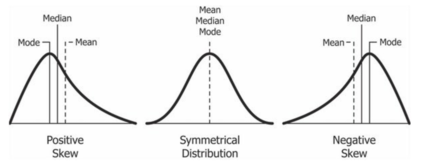
\includegraphics[scale=1.5]{SkewedData} \\
Data can also be bimodal, meaning it has two peaks \\
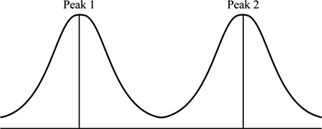
\includegraphics[scale=0.7]{Bimodal} \\

\section*{Measures of Central Tendency}
There are four measures of central tendency that we should be aware of:
\begin{itemize}
	\item Mode - The mode is the value that occurs most frequently. The distribution is uni-modal if there is only one mode. If two non-adjacent values occur mode frequently than the rest, the distribution is said to be bi-modal, even if the frequencies aren't the same. 
	\item Medial - It is the middle value. It is a good measure as it isn't skewed as much by outliers but most representative for symmetrical data. 
	\item Mean - Found by adding all the values together and dividing by the number of values. We use the symbol $\bar{x}$ to denote the mean. It is the best measure for skewed data but also representative for symmetrical data. It is affected by outliers. 
	\item Midrange - This is the average of the highest and lowest values. It is easy to calculate but only useful when the data is symmetrical and contains no outliers. 
\end{itemize}

\section*{Measures of Spread}
There are three measures of spread we need to know about which help us talk about how varied the data is.
\begin{itemize}
	\item Range - This is the highest subtract the lowest. Again this is not useful if we have any outliers.
	\item Interquartile Range - As seen before. We can also find the semi-interquartile range which is half the interquartile range.
	\item Standard Deviation - This we will learn about separately but is the most widely used measure of spread.   
\end{itemize}

\section*{Standard Deviation}
Why is it useful?
\begin{itemize}
	\item Approximately 68\% of values lie within 1 standard deviation of the mean. 
	\item 95\% lie within 2
\end{itemize}
If you have a particular values which is more than two standard deviations from the mean it should be investigated as a possible outlier. \\
\begin{align*}
\text{Sum of Squares } & = S_{xx} \\ 
& = \sum x^2 - n\bar{x}^2 \\
& = \sum x^2 - \frac{(\sum x)^2}{n} \\
\end{align*}
The variance is found by $var = s^2 = \frac{s_{xx}}{n-1}$ \\
The standard deviation is found by the square root of the variance. \\
$s = \sqrt{\frac{s_{xx}}{n-1}} = \sqrt{var}$

\subsubsection*{Example 1}
Find the standard deviation of 0, 1, 0, 3, 0, 2
\begin{align*}
\bar{x} & = \frac{1 + 2 + 3}{6} = 1 \\
s_{xx} & = (0^2 + 1^2 + 0^2 + 3^2 + 0^2 + 2^2) - 6 \times 1^2
& = 14-6 = 8 \\
s & = \sqrt{\frac{s_{xx}}{n-1}} \\
& = \sqrt{\frac{8}{5}} = 1.26 \\
\end{align*}

\subsection*{Frequency tables}
If you have a frequency table, we can still work out the standard deviation. The only thing that changes is our formula for sum of squares: \\
$s_{xx} = \sum x^2f - n\bar{x}^2$ \\

\section*{Binomial Distribution}
\begin{itemize}
	\item Running as a set number of trials, n
	\item Only two possible outcomes
	\item Probability of success is p
	\item Trials are independent
\end{itemize}
$X \sim B(n,p)$ means X is binomial distributed with n trials and a probability of success p. \\
$P(X=r) = \binom{n}{r}p^r(1-p)^{n-r}$ for r successes out of n

\subsection*{Probability / Cumulative }
Binomial PD refers to the probability distribution at a single value. e.g. $P(X=a)$ \\
Binomial CD refers to the cumulative distribution e.g. $P(X \leqslant a)$\\

\section*{Normal Distribution}
All normal curves are governed by 2 parameters: The mean ($\mu$) and the standard deviation ($\sigma$). They are symmetrical about the mean and there is a point of inflection 1 s.d. away from the mean. \\

If X has a normal distribution with mean $\mu$ and variance $\sigma^2$ we write $X \sim N(\mu, \sigma^2)$. The standard normal distribution has mean 0 and variance 1. It is written $Z$, so $Z \sim N(0,1)$. \\

As normal distributions represent continuous data, it only makes sense to find the probability that $X$ takes a value in a particular interval. The probability corresponds to the area under the curve in the interval. There is no simple formula that can be used to find the probability for an interval so we use a calculator.  \\

All normal distributions can be mapped onto each other using a stretch and a shift. It is possible and easy to transform any normal distribution to a standard normal. If $X \sim N(\mu, \sigma^2)$, $Z = \frac{X - \mu}{\sigma} \sim N(0,1)$ \\

\subsection*{Working Backwards}
If we know $\mu$ and $\sigma$ and the probability, we can use the inverse normal function on a calculator to find the interval. We can also use it to form simultaneous equations which can be solved to find one or more of the variables. \\
\subsubsection*{Example 1}
A machine is designed to fill jars so that mass, $X$ follows a normal distribution with mean $\mu g$ and s.g $\sigma g$. If:
\begin{itemize}
	\item $p(X > 210) = 0.025$ 
	\item $p(X < 108) = 0.04$
\end{itemize}
Find $\mu$ and $\sigma$ to 3.s.f. \\ 

First we use the inverse normal function to go from the probabilities to a $Z$ value. With these two values we can form two equations of the form $Z = \frac{x - \mu}{\sigma}$ with the given $X$ values and calculated $Z$ values. This means that we have two equations and two unknowns and they can be solved for $\mu$ and $\sigma$ to give $\mu = 204, \sigma = 3.23$ \\
\subsection*{Approximating a Discrete Distribution Using Normal}
A continuity correction must be applied when approximating a discrete random variable (such as the binomial distribution) to a continuous distribution (such as the normal distribution). \\

We apply a continuity correction by treating each discrete bar as an interval of all the values that would round to it (e.g. 0.5 above and below). So if we want to look at $p(X=5)$ this is corrected to $p(4.5 < X < 5.5)$. 

\subsection*{Approximating the Binomial Using a Normal Distribution}
To approximate the binomial using normal we must have:
\begin{itemize}
	\item n large
	\item $0 \ll np \ll n$
\end{itemize}
If the conditions are met then $X$ can be reasonably approximated using  $X \sim N(np, npq)$ where $q = 1-p$. We need to remember to apply a continuity correction as we are going from a discrete distribution to a continuous one. \\

This is useful where $n$ is very large as the binomial distribution can become quite slow to calculate. \\
\end{document}